\documentclass[10pt]{article}
\usepackage[margin=1.6cm]{geometry}
\usepackage{amsmath,amssymb}
\usepackage{tikz}
\usetikzlibrary{positioning,arrows.meta,fit,backgrounds}
\usepackage[hidelinks]{hyperref}
\usepackage{xcolor}
\definecolor{codegray}{gray}{0.94}
\newcommand{\code}[1]{\colorbox{codegray}{\small\texttt{#1}}}
\newcommand{\Jhat}{\hat{J}}
\newcommand{\Hhat}{\hat{H}}
\pagestyle{empty}
\setlength{\parindent}{0pt}
\setlength{\parskip}{4pt}

\begin{document}

\begin{center}
    {\LARGE\bfseries Hamiltonian ROMs in NiTROM-v2}\\[2pt]
    {\small Port of the symplectic integrators, Hamiltonian latent model, and
    variationally consistent projection --- September 30, 2026}
\end{center}

\textbf{Setting.}\; The latent dynamics derive from a polynomial Hamiltonian.
With trial basis $\Phi \in \mathbb{R}^{n\times r}$ and canonical-type
full-order symplectic structure $J = -J^\top = J^{-\top}$, $JJ = -I$
(validated at construction; the reduced $\Jhat$ is non-canonical and only
skew),
\begin{equation*}
    \Hhat(z) \;=\; \tfrac12\, z^\top A_2 z \;+\; \tfrac13\, A_3(z,z,z) \;+\;\cdots,
    \qquad
    \dot z \;=\; \Jhat\,\nabla \Hhat(z),
    \qquad
    \Jhat \;=\; \Phi^\top J \Phi ,
\end{equation*}
where $\Hhat$ is the \emph{reduced} Hamiltonian --- conceptually
$\Hhat = H \circ \mathrm{decode}$, but parameterized directly by the latent
coefficient tensors $A_2, A_3, \dots$, which are trained jointly with
$\Phi$. Both $\Hhat$ and $\nabla \Hhat$ use the same $1/k$ convention (the
old code was inconsistent about this).

\begin{center}
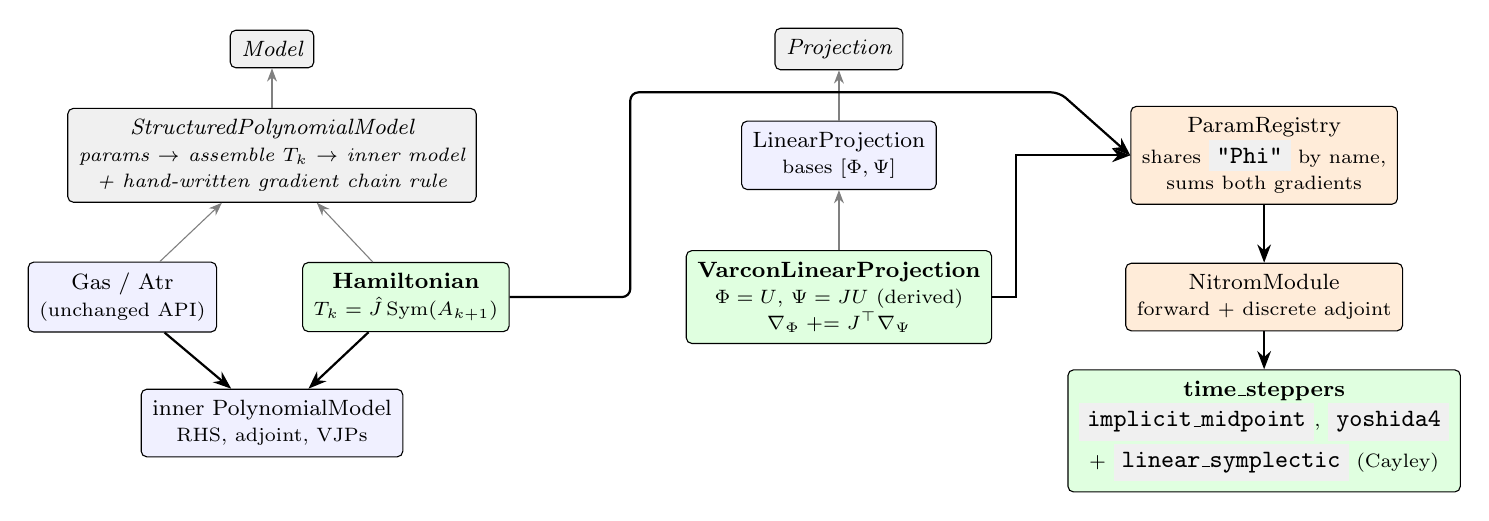
\begin{tikzpicture}[
    font=\footnotesize,
    box/.style={draw, rounded corners=2pt, fill=blue!6, inner sep=4pt, align=center},
    abs/.style={box, fill=gray!12, font=\footnotesize\itshape},
    new/.style={box, fill=green!12},
    inh/.style={-{Stealth}, gray},
    use/.style={-{Stealth}, thick}]

  % ---- left column: model hierarchy -------------------------------------
  \node[abs]                    (model) at (0, 0)     {Model};
  \node[abs]                    (spm)   at (0, -1.35) {StructuredPolynomialModel\\ \scriptsize params $\to$ assemble $T_k$ $\to$ inner model\\ \scriptsize + hand-written gradient chain rule};
  \node[box]                    (gas)   at (-1.9, -3.15) {Gas / Atr\\ \scriptsize (unchanged API)};
  \node[new]                    (ham)   at (1.7, -3.15)  {\textbf{Hamiltonian}\\ \scriptsize $T_k = \Jhat\,\mathrm{Sym}(A_{k+1})$};
  \node[box]                    (poly)  at (0, -4.75) {inner PolynomialModel\\ \scriptsize RHS, adjoint, VJPs};
  \draw[inh] (spm) -- (model);
  \draw[inh] (gas) -- (spm);
  \draw[inh] (ham) -- (spm);
  \draw[use] (gas) -- (poly);
  \draw[use] (ham) -- (poly);

  % ---- middle column: projection hierarchy ------------------------------
  \node[abs] (proj) at (7.2, 0)     {Projection};
  \node[box] (lin)  at (7.2, -1.35) {LinearProjection\\ \scriptsize bases $[\Phi,\Psi]$};
  \node[new] (var)  at (7.2, -3.15) {\textbf{VarconLinearProjection}\\ \scriptsize $\Phi = U$, $\Psi = J U$ (derived)\\ \scriptsize $\nabla_\Phi \mathrel{+}= J^\top \nabla_\Psi$};
  \draw[inh] (lin) -- (proj);
  \draw[inh] (var) -- (lin);

  % ---- right column: registry, module, steppers -------------------------
  \node[box, fill=orange!15] (reg) at (12.6, -1.35) {ParamRegistry\\ \scriptsize shares \code{"Phi"} by name,\\ \scriptsize sums both gradients};
  \node[box, fill=orange!15] (mod) at (12.6, -3.15) {NitromModule\\ \scriptsize forward + discrete adjoint};
  \node[new]                 (ts)  at (12.6, -4.85) {\textbf{time\_steppers}\\ \scriptsize \code{implicit\_midpoint}, \code{yoshida4}\\ \scriptsize + \code{linear\_symplectic} (Cayley)};
  \draw[use] (var.east) -- ++(3mm,0) |- (reg.west);
  \draw[use, rounded corners=3pt]
      (ham.east) -- (4.55, -3.15) -- (4.55, -0.55) -- (10.0, -0.55)
      -- (reg.west);
  \draw[use] (reg) -- (mod);
  \draw[use] (mod) -- (ts);
\end{tikzpicture}
\end{center}

\textbf{1.\ Symplectic integrators}\;
(\code{time\_steppers/time\_stepper.py}).\;
Implicit midpoint is the 1-stage Gauss tableau; Yoshida-4 is its triple-jump
composition with substeps $(\gamma_1, \gamma_2, \gamma_1)$, written as a
3-stage \emph{diagonally implicit} RK tableau. Because both are plain Butcher
tableaus, the existing Newton stage solve, dense solver, and \emph{discrete
adjoint} work unchanged (verified orders $2.00$ and $4.00$). For linear
dynamics $\dot z = A z$, \code{linear\_symplectic.py} adds the exact Cayley
propagator $C(h) = (I - \tfrac h2 A)^{-1}(I + \tfrac h2 A)$ (dense
numpy/torch; sparse via \code{splu}, numpy only); the backward adjoint march
uses the transposed propagators.

\textbf{2.\ Hamiltonian model}\;
(\code{latent\_space\_models/hamiltonian\_polynomial\_model.py}).\;
The delegation skeleton of the GAS model was extracted into the abstract
\code{StructuredPolynomialModel}; GAS/ATR and the new model subclass it.
The Hamiltonian model assembles $T_k = \Jhat\,\mathrm{Sym}(A_{k+1})$
into the inner polynomial model and chains gradients back:
$\nabla_{A_{k+1}} = \mathrm{Sym}^\top(\Jhat^\top G_k)$ and
$\nabla_\Phi = J\Phi\, \nabla_{\Jhat}^{\top} + J^\top\!\Phi\, \nabla_{\Jhat}$
from $\delta\Jhat = \delta\Phi^\top(J\Phi) + (\Phi^\top J)\delta\Phi$.
Parameter order: $[A_2, A_3, \Phi]$. No forcing (autonomous).

\textbf{3.\ Variationally consistent projection}\;
(\code{projections/varcon\_linear\_projection.py}).\;
Simply calls \code{LinearProjection} with bases $[U,\, JU]$: encoder $(JU)^\top$, decoder
$U (U^\top J^\top U)^{-1}$, so encode$\,\circ\,$decode $=$ Id. Only
\code{"Phi"} is free ($\Psi$ is derived), and the VJPs fold the $\Psi$
gradient back through $\delta\Psi = J\,\delta\Phi$. \emph{Note:} $r$ must be
even --- $U^\top J^\top U$ is skew and singular for odd $r$. The registry
then shares $\Phi$ with the model automatically.

\textbf{Gradient of the shared basis.}\;
The registry sums three labeled contributions into the total gradient of the
training cost w.r.t.\ $U \equiv \Phi$ (derivation on the next page):
\begin{equation*}
    \nabla_U \mathcal{L}
    \;=\;
    \underbrace{\nabla^{\mathrm{dec}}_{\Phi}
        + J^\top \nabla^{\mathrm{dec}}_{\Psi}}_{\text{(a) reconstruction (decoder)}}
    \;+\;
    \underbrace{J\Phi\, \nabla_{\Jhat}^{\top}
        + J^\top \Phi\, \nabla_{\Jhat}}_{\text{(b) dynamics through} \Jhat}
    \;+\;
    \underbrace{J^\top \nabla^{\mathrm{enc}}_{\Psi}}_{\text{(c) ICs (encoder)}},
    \quad
    \nabla_{\Jhat} \;=\; \sum_k \bigl\langle G_k,\,
        \mathrm{Sym}(A_{k+1}) \bigr\rangle_{\text{trailing}},
\end{equation*}
where $G_k$ are the discrete-adjoint gradients w.r.t.\ the assembled inner
tensors $T_k$, and each $J^\top \nabla_\Psi$ term folds the derived test
basis $\Psi = J\Phi$ back onto $\Phi$.

\textbf{4.\ Tests}\;
(860 total, 140 new; all pass).\; Input/shape validation on every new class,
including that $J$ is canonical-type while $\Jhat$ is only skew;
VJPs vs.\ torch autograd \emph{and} central finite differences, including a
cubic-only case isolating the slot-symmetrization adjoint (where the old code
had a bug); convergence orders; symplecticity $M^\top J M = J$;
Cayley-vs-tableau agreement; exact conservation of quadratic $H$ over long
horizons and bounded (non-secular) drift for cubic $H$; and the decisive
end-to-end check, discrete adjoint vs.\ finite differences through the full
shared-$\Phi$ pipeline (\code{tests/optimization/modules/test\_nitrom\_hamiltonian.py}).


\newpage

\begin{center}
    {\Large\bfseries Appendix: the shared-basis gradient, from the Lagrangian}
\end{center}

The training gradient originates from the adjoint (Lagrangian) formulation
(one trajectory shown; $U \equiv \Phi$):
\begin{equation*}
    \mathcal{L}(U, A_2, A_3)
    \;=\;
    \underbrace{\textstyle\sum_{ij}\mathcal{J}_{ij}}_{\text{(a) misfit}}
    \;+\;
    \underbrace{\int_{t_0}^{t_i} \lambda^\top\bigl(\dot z
        - \Jhat\,\nabla\Hhat(z)\bigr)\,\mathrm{d}t}_{\text{(b) dynamics}}
    \;+\;
    \underbrace{\lambda_0^\top\bigl(z_0 - (JU)^\top x_0\bigr)}_{\text{(c) initial condition}} .
\end{equation*}
$U$ appears in exactly three places, each yielding one contribution to
$d\mathcal{L}/dU$: in (a) through the decoder
$\hat x = U (U^\top J^\top U)^{-1} z$; in (b) through
$\Jhat = U^\top J U$, where
$\delta\Jhat = \delta U^\top (JU) + (U^\top J)\,\delta U$ gives
\begin{equation*}
    \partial_U^{(\mathrm b)}\mathcal{L}
    = J U\, \nabla_{\Jhat}^{\top} + J^\top U\, \nabla_{\Jhat},
    \qquad
    \nabla_{\Jhat} = -\!\int \lambda\, \nabla\Hhat(z)^\top \mathrm{d}t
    \;\;\widehat{=}\;\; \sum_k \bigl\langle G_k, \mathrm{Sym}(A_{k+1})
    \bigr\rangle_{\text{trailing}},
\end{equation*}
with $G_k$ the discrete-adjoint accumulations of
$\lambda \otimes z \otimes \cdots \otimes z$ (the $A_k$ gradients come from
the same term via $\partial_{A_{k+1}}$); and in (c) directly,
$\partial_U^{(\mathrm c)}\mathcal{L} = -J^\top x_0 \lambda_0^\top$.

\emph{Where do the $\nabla_\Psi$ partials come from, if everything depends on
$U$ alone?}\; They are an artifact of the implementation's parameterization,
not extra physics. The generic \code{LinearProjection} treats $\Phi, \Psi$ as
\emph{independent} (encode $= \Psi^\top q$, decode $= \Phi S z$ with
$S = (\Psi^\top\Phi)^{-1}$) and its VJPs return the pair of partials
$\bigl(\partial\mathcal{L}/\partial\Phi\big|_\Psi,\,
\partial\mathcal{L}/\partial\Psi\big|_\Phi\bigr)$. The varcon subclass
imposes $\Psi = J\Phi$ and applies the chain rule
\begin{equation*}
    \frac{d\mathcal{L}}{dU}
    = \frac{\partial\mathcal{L}}{\partial\Phi}\bigg|_{\Psi}
    + J^\top\, \frac{\partial\mathcal{L}}{\partial\Psi}\bigg|_{\Phi} ,
    \qquad\text{so}\qquad
    \nabla_U \mathcal{L}
    = \underbrace{\nabla^{\mathrm{dec}}_{\Phi}
        + J^\top \nabla^{\mathrm{dec}}_{\Psi}}_{\text{(a) reconstruction}}
    + \underbrace{J\Phi\, \nabla_{\Jhat}^{\top}
        + J^\top \Phi\, \nabla_{\Jhat}}_{\text{(b) dynamics}}
    + \underbrace{J^\top \nabla^{\mathrm{enc}}_{\Psi}}_{\text{(c) init.\ cond.}} .
\end{equation*}
The encoder $\Psi^\top x_0$ contains no explicit $\Phi$, so its $\Phi$-partial
vanishes and $J^\top \nabla_\Psi^{\mathrm{enc}} = J^\top x_0 \lambda_0^\top$
reproduces (c) exactly. The decoder, in the split view, depends on
\emph{both} ($\Phi$ as leading factor and inside $S$; $\Psi$ inside $S$), and
the sum of its two chained partials equals $d/dU$ of
$U(U^\top J^\top U)^{-1}$ --- the identity pinned against autograd in the
projection tests.

\end{document}
